%%%INTRODUCCIÓN GENERAL%%%
\chapter*{Introducción}
\addcontentsline{toc}{chapter}{Introducción}

El prefijo nano deriva del griego \emph{nanos}, que significa literalmente ``enano''. En el sistema internacional de unidades, el prefijo nano representa un factor de $\mathrm{10^{-9}}$, o una mil millonésima parte. Al añadir este prefijo a la unidad de longitud, obtenemos ``nanómetro'' (nm), o una mil millonésima parte de un metro. Así la nanotecnología se define como la ciencia, tecnología, e ingeniería que trata sistemas en el rango aproximado de 1-100 nanómetros. \citep{Haick2013,Gressler2013}. Se ha de tener claro en que rango de dimensiones se encuentra la escala nanométrica, los seres humanos estamos acostumbrados a escalas grandes, se nos hace fácil entender las comparaciones de kilómetros con metros, o milímetros con metros, pero al reducir el tamaño a micrómetros nos cuesta, pues son escalas que se escapan de nuestros sentidos. Un micrómetro es a un metro como un kilómetro es a un milímetro, teniendo eso en cuenta, un nanómetro es a un milímetro, como un micrómetro es a un kilómetro. La figura \ref{fig:scale} muestra una escala de tamaños con varios ejemplos desde la escala humana hasta la atómica, la nanoescala comprende aproximadamente desde los cientos de nanómetros hasta fracciones de nanómetros.

\begin{figure}[h!]
	\centering
	\fbox{
		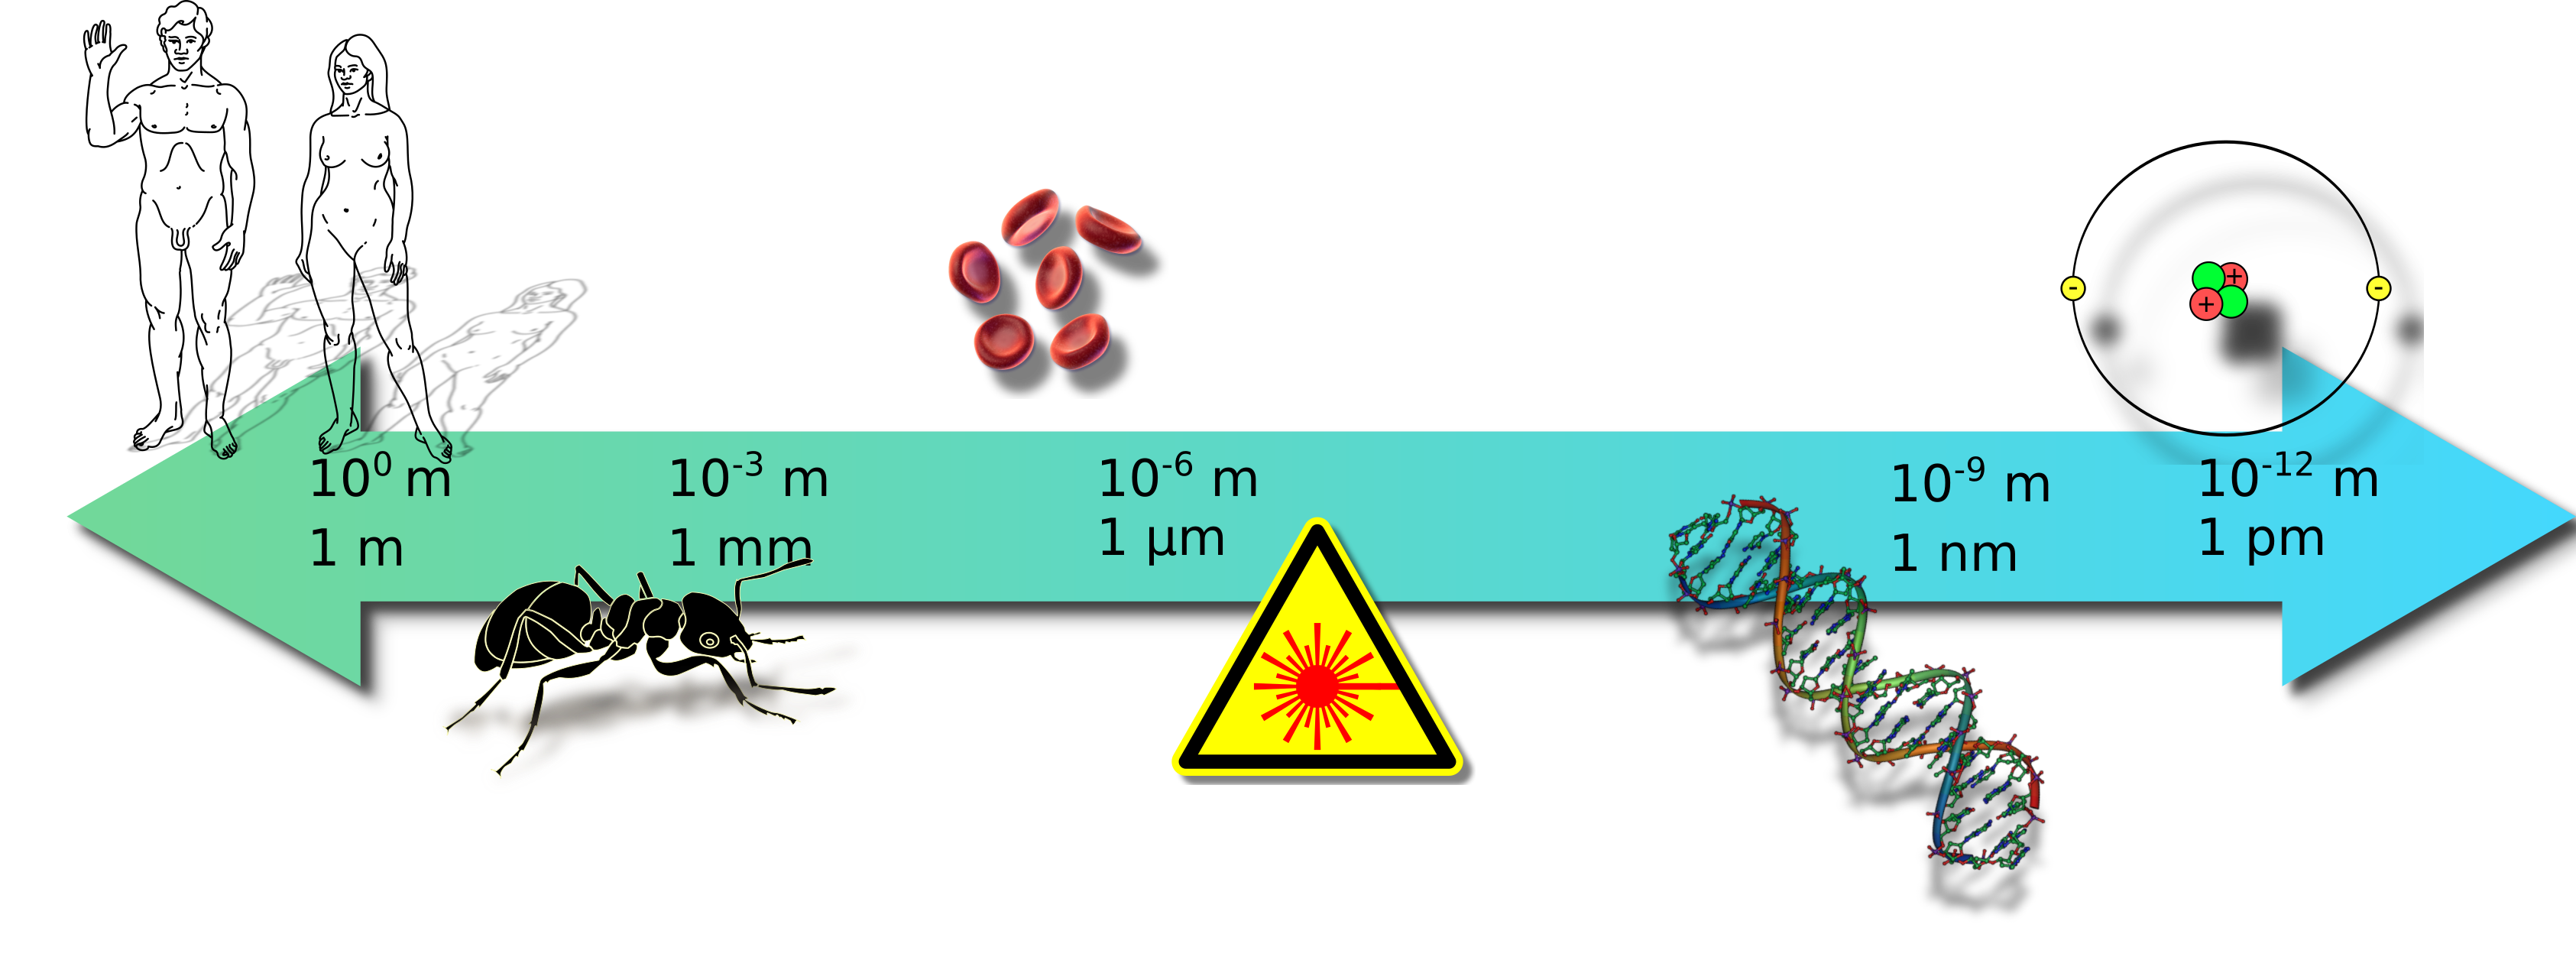
\includegraphics[width=\textwidth]{scale.png}
	}
	\caption[Comparativa de ódenes de magnitud desde metros hasta picometros]{Comparativa de órdenes de magnitud. De izquierda a derecha: Escala humana 1-2 m. Insectos 10 cm - 1 mm. Glóbulos rojos 6 $\mathrm{\mu}$m. Longitud de onda de luz visible 780-380 nm. Doble hélice de ADN 2 nm. Radio atómico de un átomo de helio 31 pm.}
\label{fig:scale}
\end{figure}

La idea de la nanotecnología fue vislumbrada por el físico Richard Feynman y expuesta en su charla \emph{``There is plenty room at the bottom''} \citep{Feynman1960}. Aquí Feynman plantea que no existen barreras físicas que impidan manipular sistemas nanométricos, moléculas, o incluso átomos. La era moderna de la nanotecnología comienza con el desarrollo del microscopio de efecto túnel por Binning y Rohrer en 1981 \citep{Binnig1982}, que les hizo ganar el Premio Nobel de Física en 1986. Un microscopio de efecto túnel (STM por sus siglas en inglés \emph{Scanning Tunneling Microscope}), puede superar resoluciones de 0,1 nm de resolución lateral, y 0,01 nm en profundidad, y trabajar en variadas condiciones, sin necesidad de alto vacío o bajas temperaturas. Además de poder resolver átomos, el STM también puede manipularlos \citep{Chen2008}.

\begin{figure}
	\centering
	\fbox{
		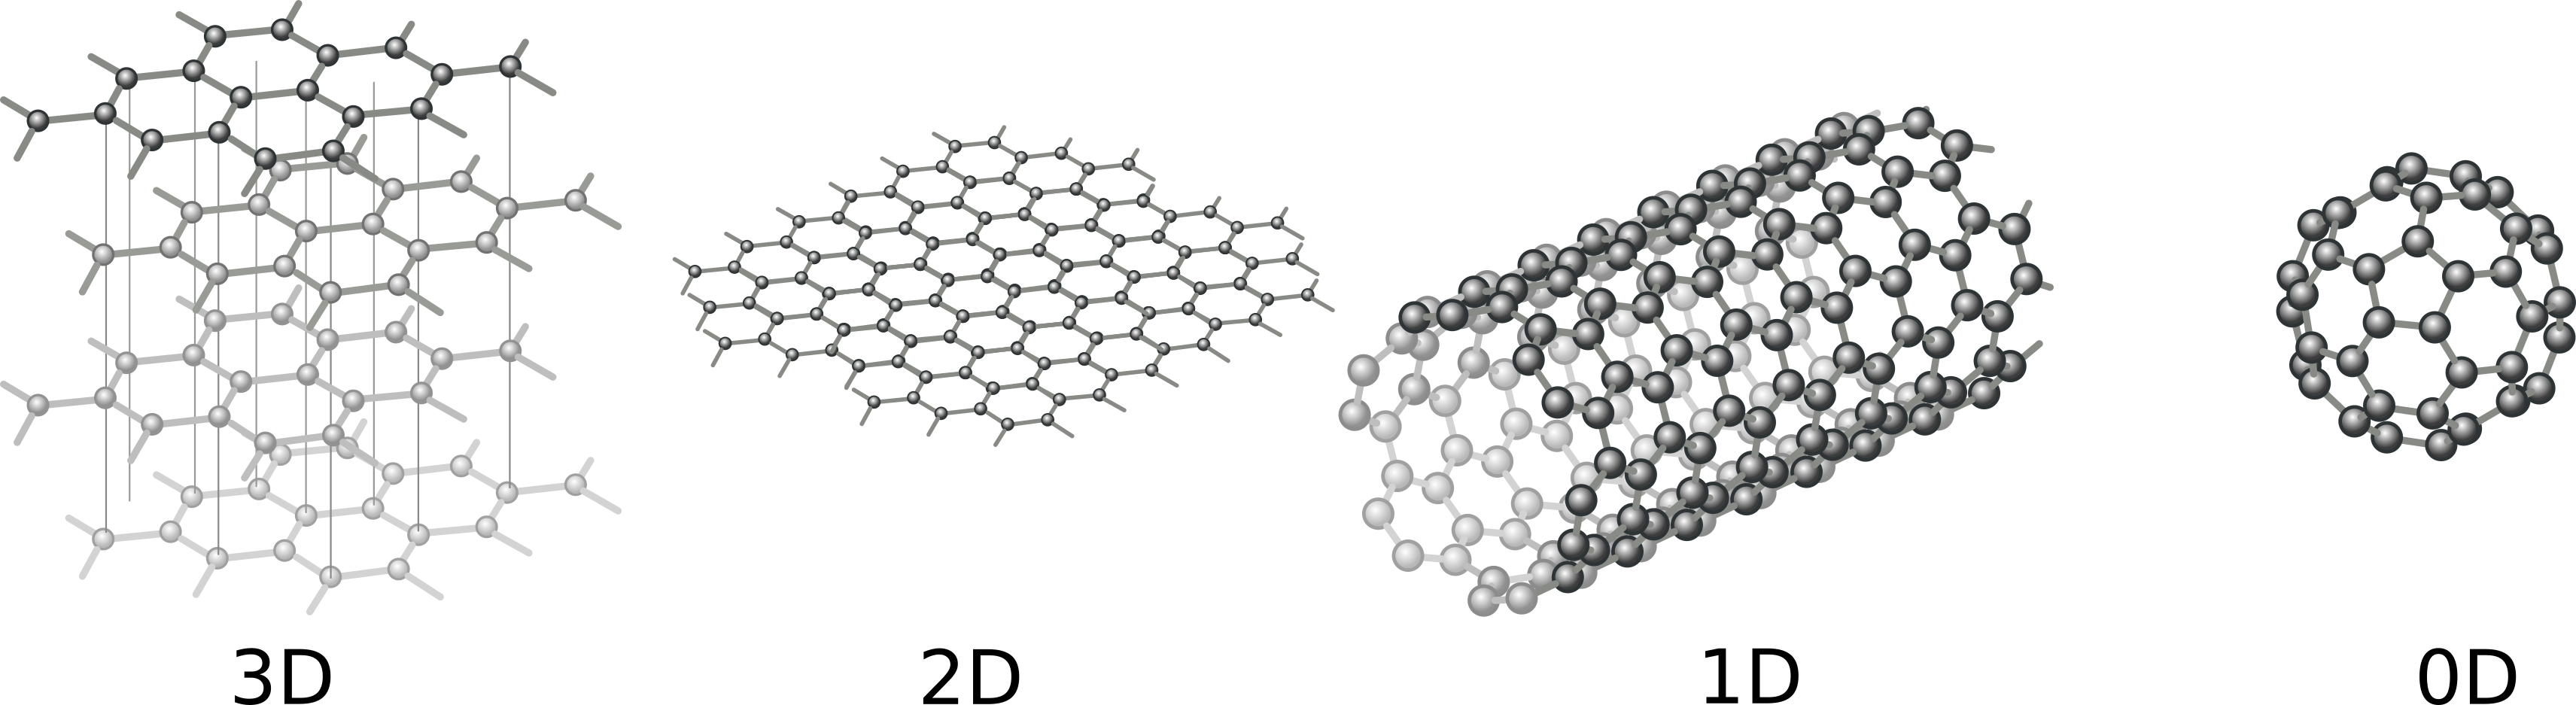
\includegraphics[width=\textwidth]{carbon_alotropes.png}
		}
	\caption[Alótropos del carbono mostrando las diferentes dimensionalidades de los nanomateriales]{Alótropos del carbono como representación de las diferentes dimensionalidades en los nanomateriales. De izquierda a derecha: Grafito, no es un material nanoestructurado, a pesar de estar formado por varios capas de grafeno. Grafeno, solo un átomo de espesor, es un material 2D. Nanotubo de carbono, es un material 1D. Fulereno, es un material 0D.}
	\label{fig:carbon_allotropes}
\end{figure}

\section*{La física de sistemas nanométricos}


%CONFINAMIENTO cuántico
Al reducir las dimensiones a escalas nanométricas, surgen efectos de confinamiento cuántico, pues se restringe el movimiento de los electrones en el material, esto conlleva a la discretización de los niveles de energía de los electrones y al cambio de la densidad de estados del material. 


%DENSIDAD de estados en diferentes dimensiones
Dependiendo de cuantas dimensiones son llevadas a la nanoescala, es como se ve afectada la densidad de estados.

\begin{figure}[h!]
	\centering
	\fbox{
		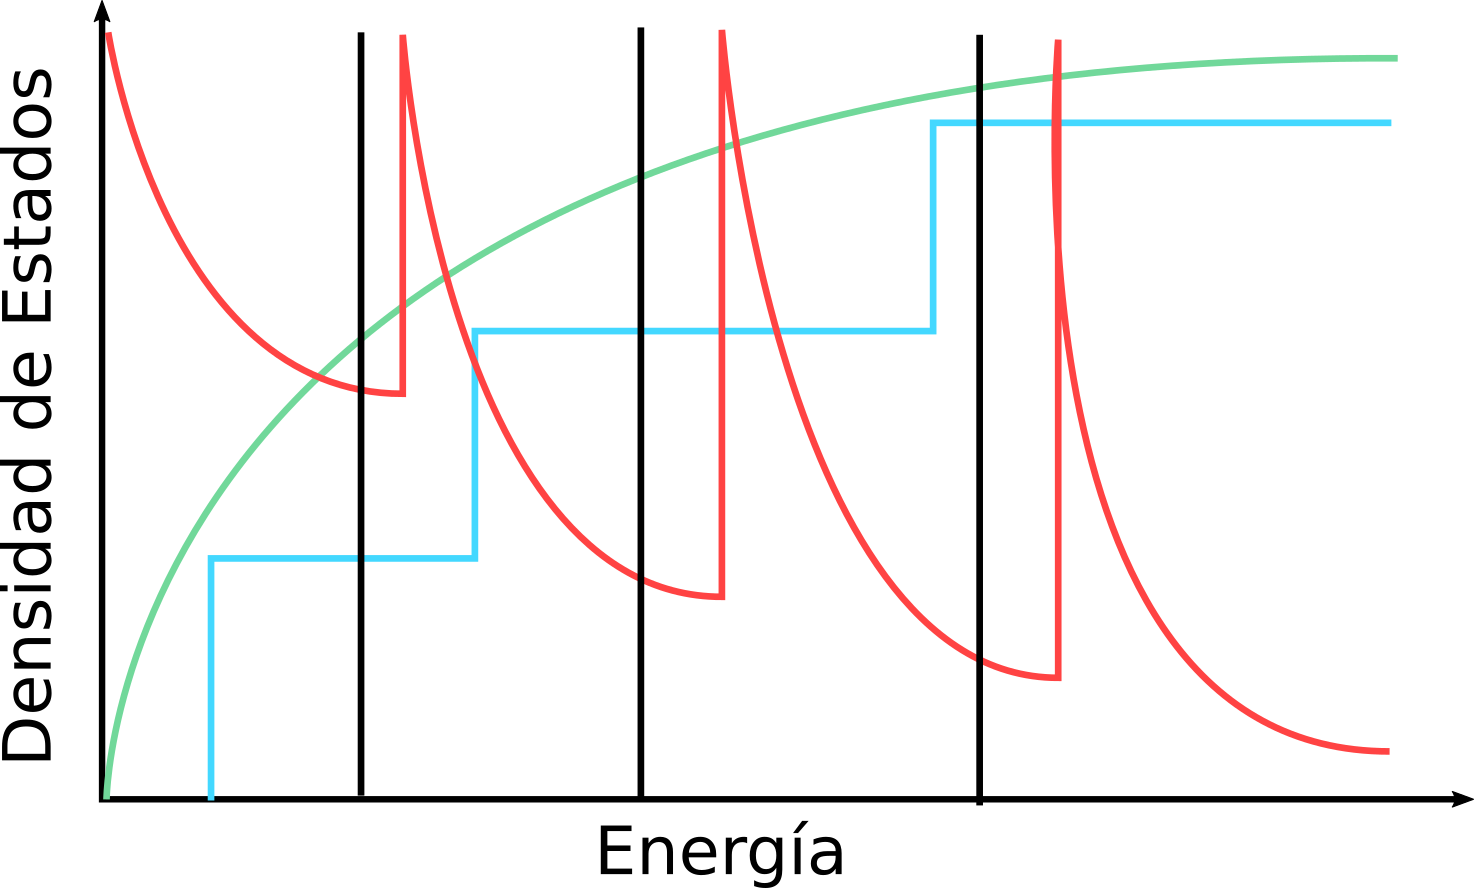
\includegraphics[width=0.6\textwidth]{DoE.png}
	}
	\caption[Densidad de estados en diferentes dimensionalidades]{Densidad de estados diferentes dimensiones. Para materiales 3D (no nanoestructurados), la densidad de estados es continua. En nanomateriales 2D, la densidad de estado forma escalones. Para materiales 1D, ésta es}
	\label{fig:DoE}
\end{figure}

%AREA superficial
Al dividir un volumen en partículas más pequeñas, el área superficial aumenta. Por ejemplo, en la secuencia de la figura \ref{fig:area_cubes}, el volumen total en cada división no cambia, pero el área superficial se dobla \footnotemark, siguiendo está lógica, al reducir un cubo de lado 1 cm a 100 nm, el área total habrá aumentado 100.000 veces. El aumento del área superficial aumenta la reactividad del material, ya que hay más lugar para, por ejemplo, reacciones químicas. Otra forma de verlo, es considerar la proporción de átomos en la superficie, con la cantidad de átomos del interior (proporción de área superficial al volumen), esta proporción aumenta al disminuir el tamaño de las partículas.

\footnotetext{Si en la secuencia de la figura \ref{fig:area_cubes} el cubo más grande tiene lado $l$, su área superficial es $6 \times l^2$, en la primera división, el lado de cada cubo es $l/2$ y el área de cada uno es $6\left( l/2\right)^2$, que en total hacen $6\left(l/2\right)^2\times 8$, en la segunda división el área total es $6\left(l/4\right)^2\times 8 \times 8$, así, en la n-ésima división el área es $6l^2 \left(1/2^n\right)^2\times 8^n$ o $6l^2 \times 2^n$. Así, el área superficial se dobla con cada división.}

\begin{figure}[h!]
	\centering
	\fbox{
		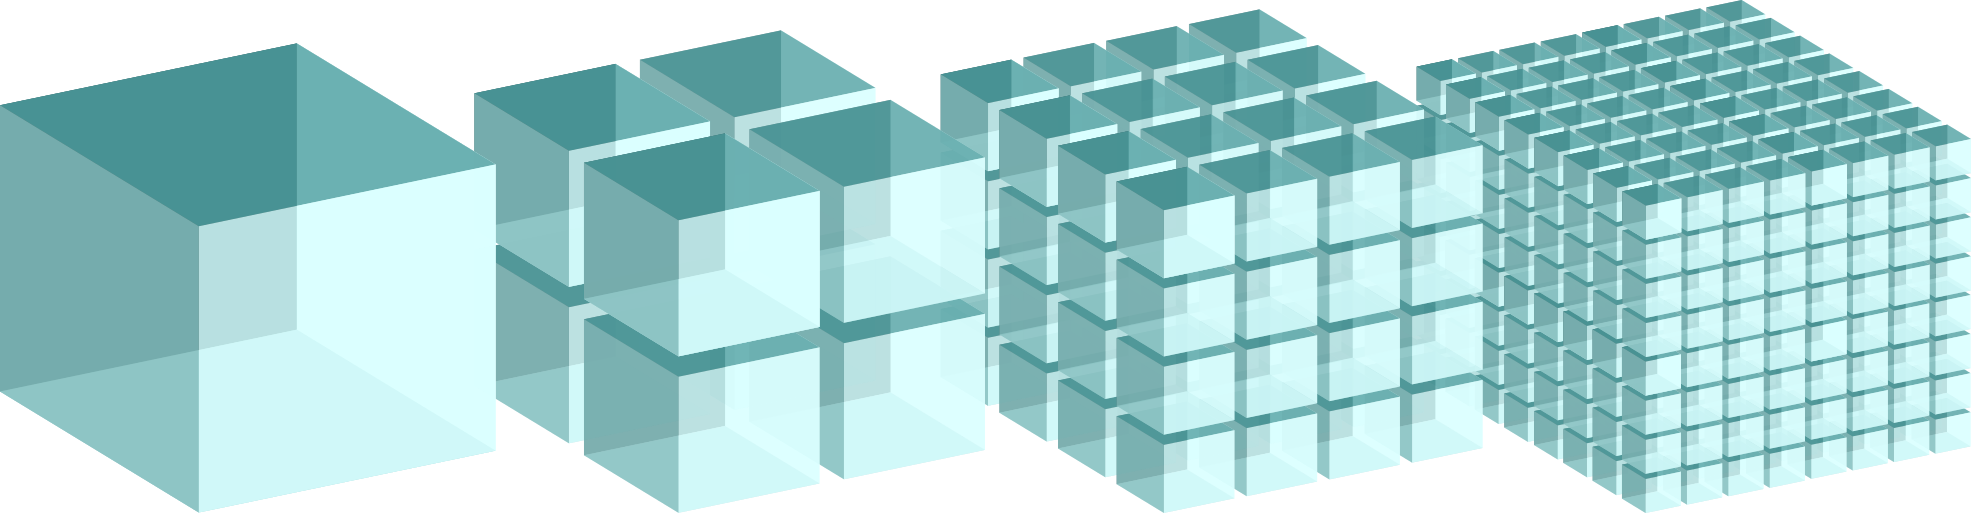
\includegraphics[width=\textwidth]{area_cubes.png}
		}
	
	\caption[Subdivisiones de un cubo demostrando el aumento de área superficial total]{Secuencia de divisiones de un cubo conservando el volumen (cantidad de material). Si se comienza con un cubo de 1 cm de lado y se subdivide hasta tener cubos de 100 nm de lado, el área superficial total pasaría de 6 $\mathrm{cm^2}$ a 60 $\mathrm{m^2}$.}
	\label{fig:area_cubes}
\end{figure}
